%% Copyright (C) 2010, Gostai S.A.S.
%%
%% This software is provided "as is" without warranty of any kind,
%% either expressed or implied, including but not limited to the
%% implied warranties of fitness for a particular purpose.
%%
%% See the LICENSE file for more information.

\chapter{Glossary}
\label{sec:glossary}

This chapter aggregates the definitions used in the this document.

\begin{description}
\item[Gostai Console] This tool provide a graphical user interface for
  Windows users to a remote \urbi server (see
  \autoref{fig:gostai-console}).  Unix users, GNU/Linux or Mac OS X,
  can use the traditional \command{telnet} tool.  Windows users are
  invited to use Gostai Console instead.  See
  \autoref{sec:tut:started}.

  \begin{figure}[htp]
    \centering
    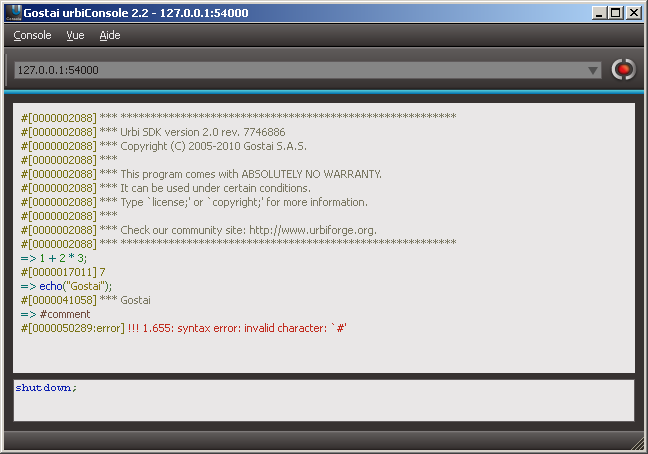
\includegraphics[width=.8\linewidth]{img/urbi-console}
    \caption{Gostai Console}
    \label{fig:gostai-console}
  \end{figure}


\item[Gostai Lab] This tool (see \autoref{fig:gostai-lab}), which
  includes the features of Gostai Console, allows to build easily
  elaborate remote controller for robots.  It provides various widgets
  to visualize data from the robot (including video and sound), and to
  modify the state of the robot.

  \begin{figure}[htp]
    \centering
    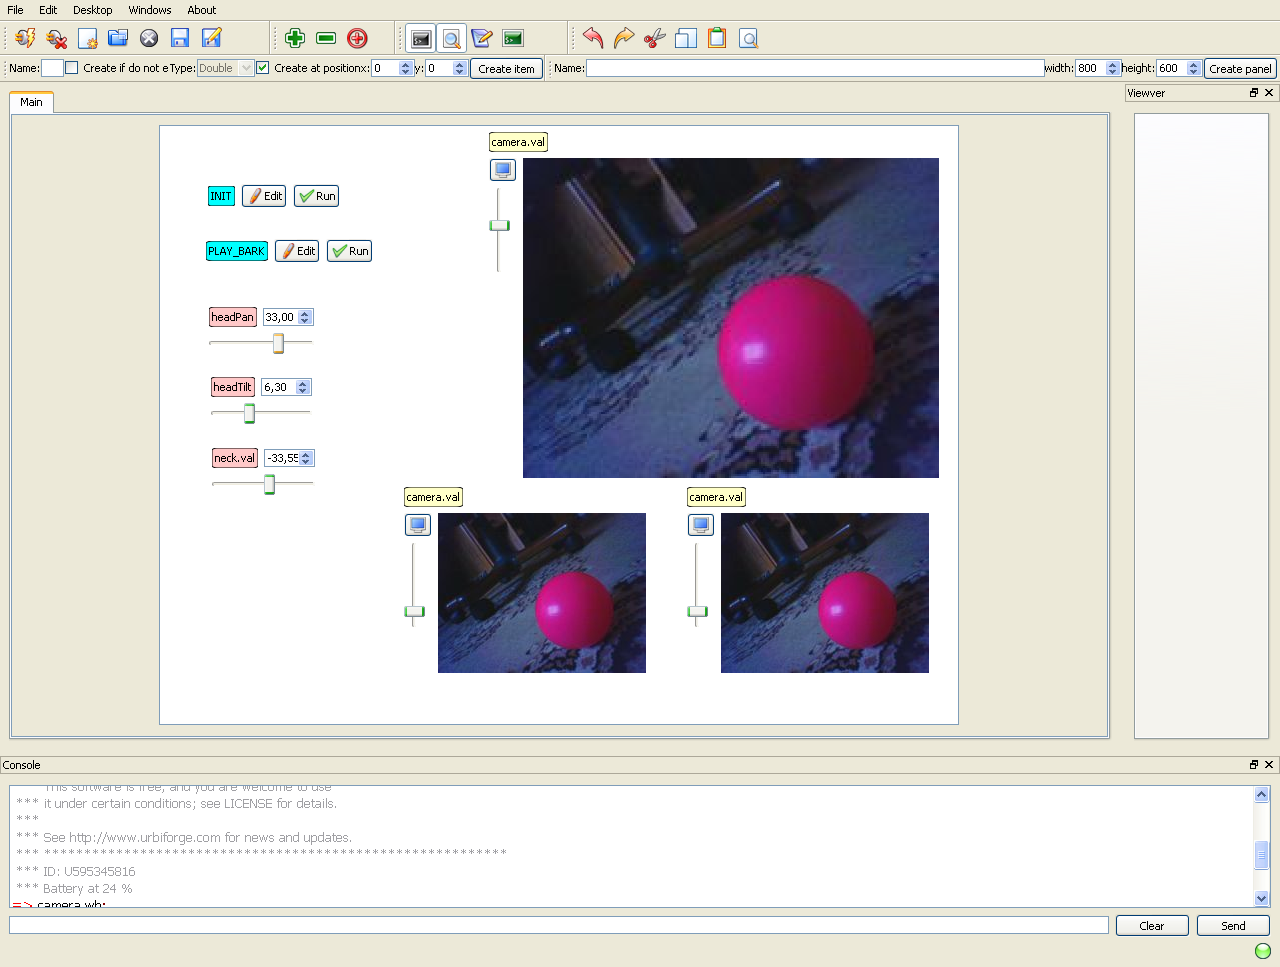
\includegraphics[width=.8\linewidth]{img/gostai-lab}
    \caption{Gostai Lab}
    \label{fig:gostai-lab}
  \end{figure}

\item[Gostai Studio] This tool (see \autoref{fig:gostai-studio}),
  includes all the features of Gostai Console and Gostai Lab.  It is a
  high-level Integrated Development Environment for \urbi.  Its
  formalism is based on \dfn{Hierarchical Finite State Machines}.

  \begin{figure}[htp]
    \centering
    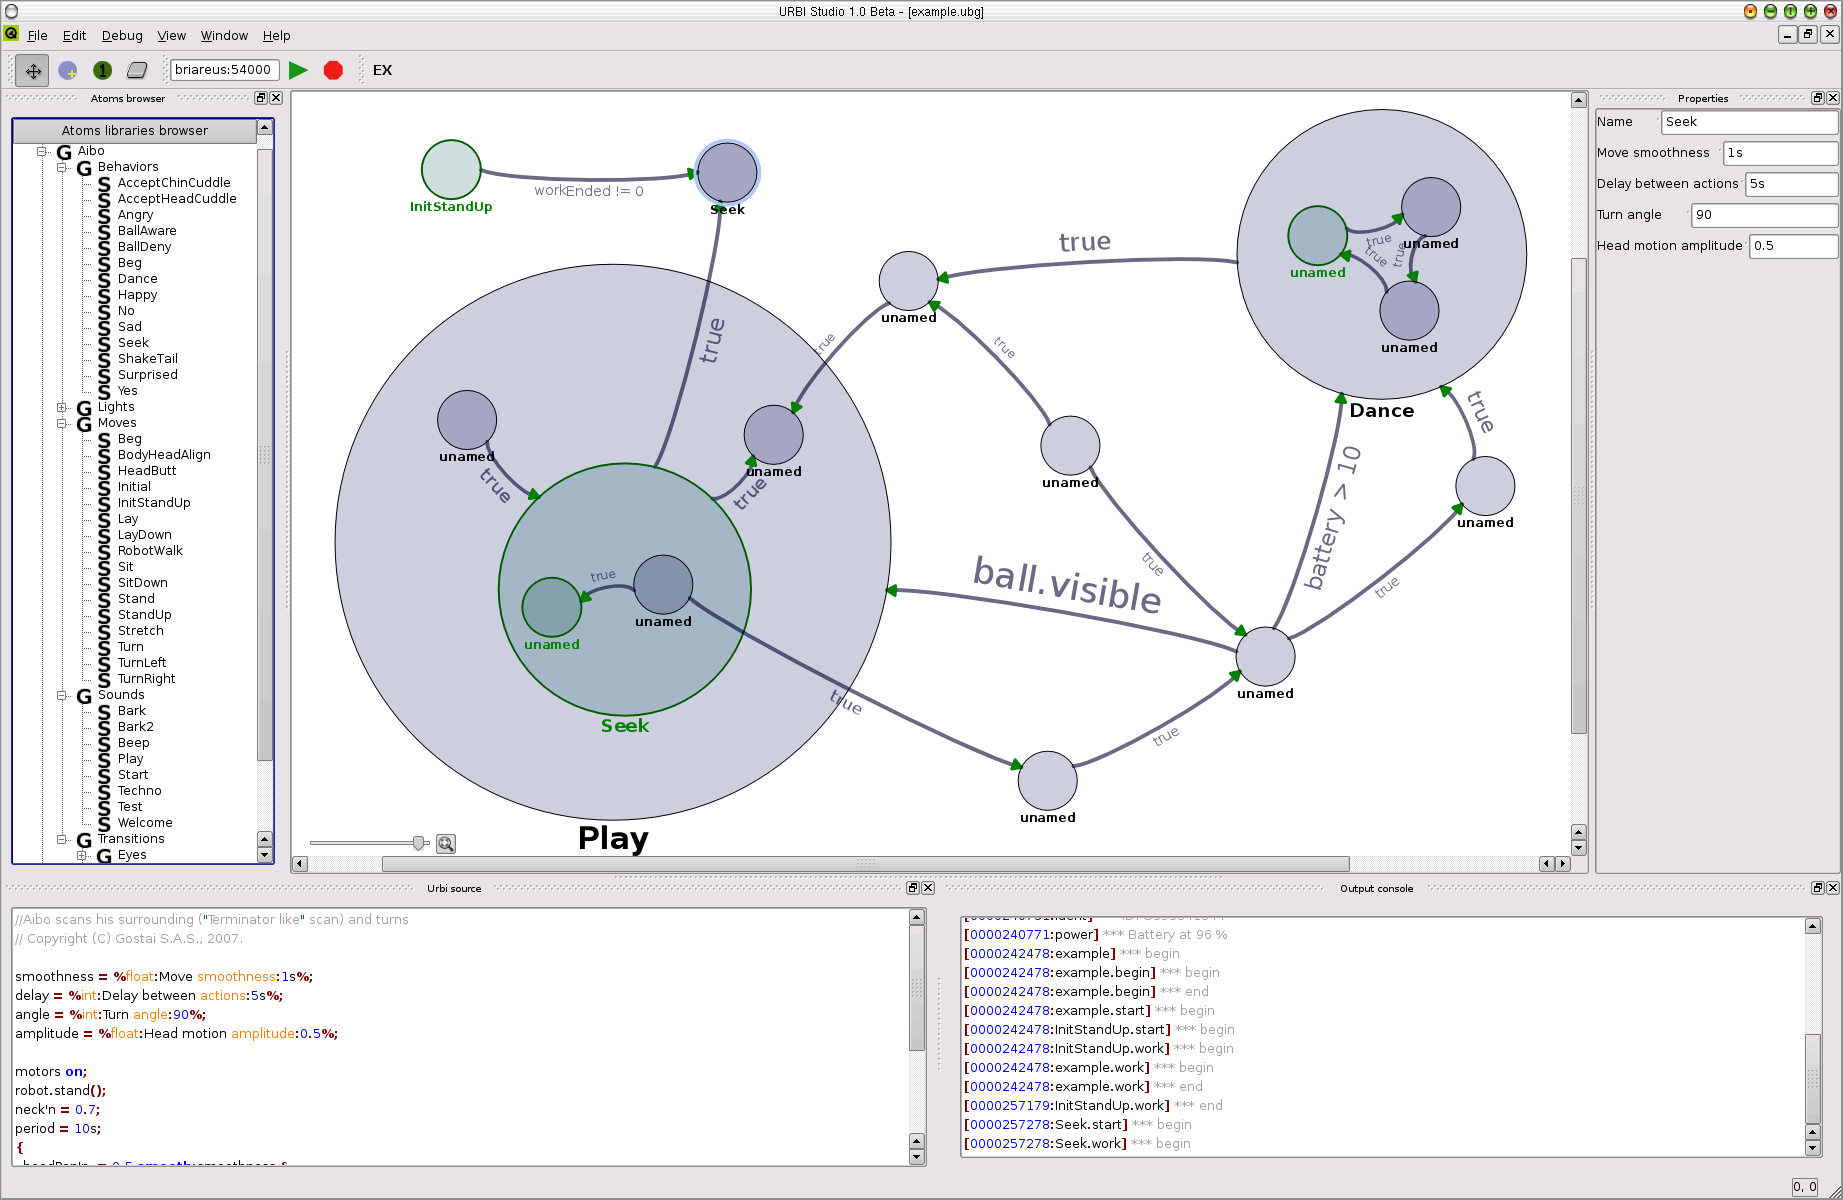
\includegraphics[width=.8\linewidth]{img/gostai-studio}
    \caption{Gostai Studio}
    \label{fig:gostai-studio}
  \end{figure}

\item[urbi-console] This is the former name of ``Gostai Console''.
  See that item.
\end{description}

%%% Local Variables:
%%% mode: latex
%%% TeX-master: "urbi-sdk"
%%% ispell-dictionary: "american"
%%% ispell-personal-dictionary: "../urbi.dict"
%%% fill-column: 76
%%% End:
